\documentclass{scrartcl}\usepackage[]{graphicx}\usepackage[]{color}
%% maxwidth is the original width if it is less than linewidth
%% otherwise use linewidth (to make sure the graphics do not exceed the margin)
\makeatletter
\def\maxwidth{ %
  \ifdim\Gin@nat@width>\linewidth
    \linewidth
  \else
    \Gin@nat@width
  \fi
}
\makeatother

\definecolor{fgcolor}{rgb}{0.345, 0.345, 0.345}
\newcommand{\hlnum}[1]{\textcolor[rgb]{0.686,0.059,0.569}{#1}}%
\newcommand{\hlstr}[1]{\textcolor[rgb]{0.192,0.494,0.8}{#1}}%
\newcommand{\hlcom}[1]{\textcolor[rgb]{0.678,0.584,0.686}{\textit{#1}}}%
\newcommand{\hlopt}[1]{\textcolor[rgb]{0,0,0}{#1}}%
\newcommand{\hlstd}[1]{\textcolor[rgb]{0.345,0.345,0.345}{#1}}%
\newcommand{\hlkwa}[1]{\textcolor[rgb]{0.161,0.373,0.58}{\textbf{#1}}}%
\newcommand{\hlkwb}[1]{\textcolor[rgb]{0.69,0.353,0.396}{#1}}%
\newcommand{\hlkwc}[1]{\textcolor[rgb]{0.333,0.667,0.333}{#1}}%
\newcommand{\hlkwd}[1]{\textcolor[rgb]{0.737,0.353,0.396}{\textbf{#1}}}%

\usepackage{framed}
\makeatletter
\newenvironment{kframe}{%
 \def\at@end@of@kframe{}%
 \ifinner\ifhmode%
  \def\at@end@of@kframe{\end{minipage}}%
  \begin{minipage}{\columnwidth}%
 \fi\fi%
 \def\FrameCommand##1{\hskip\@totalleftmargin \hskip-\fboxsep
 \colorbox{shadecolor}{##1}\hskip-\fboxsep
     % There is no \\@totalrightmargin, so:
     \hskip-\linewidth \hskip-\@totalleftmargin \hskip\columnwidth}%
 \MakeFramed {\advance\hsize-\width
   \@totalleftmargin\z@ \linewidth\hsize
   \@setminipage}}%
 {\par\unskip\endMakeFramed%
 \at@end@of@kframe}
\makeatother

\definecolor{shadecolor}{rgb}{.97, .97, .97}
\definecolor{messagecolor}{rgb}{0, 0, 0}
\definecolor{warningcolor}{rgb}{1, 0, 1}
\definecolor{errorcolor}{rgb}{1, 0, 0}
\newenvironment{knitrout}{}{} % an empty environment to be redefined in TeX

\usepackage{alltt}
\usepackage[utf8]{inputenc}
\usepackage{graphicx}%GRaphiken
\usepackage{tabularx}%Tabellen!
\usepackage[english]{babel}% Zeilentrennung besser
\usepackage{url}% Urls besser
\usepackage{textcomp}% Sonderzeichen
\usepackage{helvet}% Schrift Helvetica ?
\usepackage[helvet]{sfmath}% Helvet also in Math modes
\renewcommand\familydefault{\sfdefault}
\usepackage[
	left=3cm,
	right=2cm,
	top=1.5cm,
	bottom=1cm
	,
	includeheadfoot
	]{geometry}														% Satzspiegel
\usepackage[
	round,	%(defaultage in the main file and \input ) for round parentheses;
	%square,	% for square brackets;
	%curly,	% for curly braces;
	%angle,	% for angle brackets;
	colon,	% (default) to separate multiple citations with colons;
	%comma,	% to use commas as separaters;
	authoryear,% (default) for author-year citations;
	%numbers,	% for numerical citations;
	%super,	% for superscripted numerical citations, as in Nature;
	sort,		% orders multiple citations into the sequence in which they appear in the list of 				references;
	%sort&compress,    % as sort but in addition multiple numerical citations
                   % are compressed if possible (as 3-6, 15);
	%longnamesfirst,  % makes the first citation of any reference the equivalent of
                   % the starred variant (full author list) and subsequent citations
                   %normal (abbreviated list);
	%sectionbib,      % redefines \thebibliography to issue \section* instead of \chapter*;
                   % valid only for classes with a \chapter command;
                   % to be used with the chapterbib package;
	%nonamebreak,     % keeps all the authors names in a citation on one line;
                   %causes overfull hboxes but helps with some hyperref problems.
]{natbib}											    			% Literaturverzeichnis
\usepackage{scrhack}   % kills \float@addtolists!  warning
\usepackage[pdfpagelabels,plainpages=false, pageanchor=false]{hyperref}	


%% andere Einstellungen
\linespread{1.5}% 1.5 Zeilenabstand			
\graphicspath{{fig/}}                     % path to graphics

\title{Use the GLM, Luke.}
\subtitle{}
\author{Eduard Szöcs}
\date{\today}
\IfFileExists{upquote.sty}{\usepackage{upquote}}{}
\begin{document}
\maketitle

\section{Introduction}
Not mentioned in Newman (2013). 

Sparsely in OECD Guideline. 

Canada: 'The concept is quite advanced and as yet is not widely used in environmental toxicology.'

Wang/Riffel vergleichen NP aber kein Wort über GLM.

Brock et al. empfiehlt das sampling zui verbessern um die MDD zu verkleinern, keine erwähnung von GLMs (damit erhöhen die auch die power, wie man sieht und sind kostenlos)

\subsection{Normal Model}
$$ log(Ay_i + 1) \sim N(\mu_i, \sigma^2) $$
$$ var(log(Ay_i + 1)) = \sigma^2 $$
$$ log(Ay_i + 1) = \alpha + \beta x_i $$

OR
$$ y_i^T = log(Ay_i + 1) $$
$$ y_i^T  \sim N(\mu_i, \sigma^2) $$
$$ var(y_i^T ) = \sigma^2 $$
$$ y_i^T  = \alpha + \beta x_i $$

\subsection{Generalized Linear Model}
$$ y_i \sim NB(\mu_i, \theta) $$
$$ var(y_i) = \mu_i + \mu_i^2 / \theta $$ 
$$ log(\mu_i) = \eta_i $$
$$ \eta_i = \alpha + \beta x_i $$


\section{Methods}
\subsection{Simulation scenarious}

Derzeit, muT = 1/2 muC. Deshalb nimmt die power ab mit kleiner muC (die differnz wird kleiner). Wie kann man das umgehen/besser machen?

Andere Daten/Szenarios? Siehe Wang. 
Für beta-GLM braucht man gamlss oder ?betareg? (mal vergleichen). Gamma (densities) kann glm().


\begin{figure}
  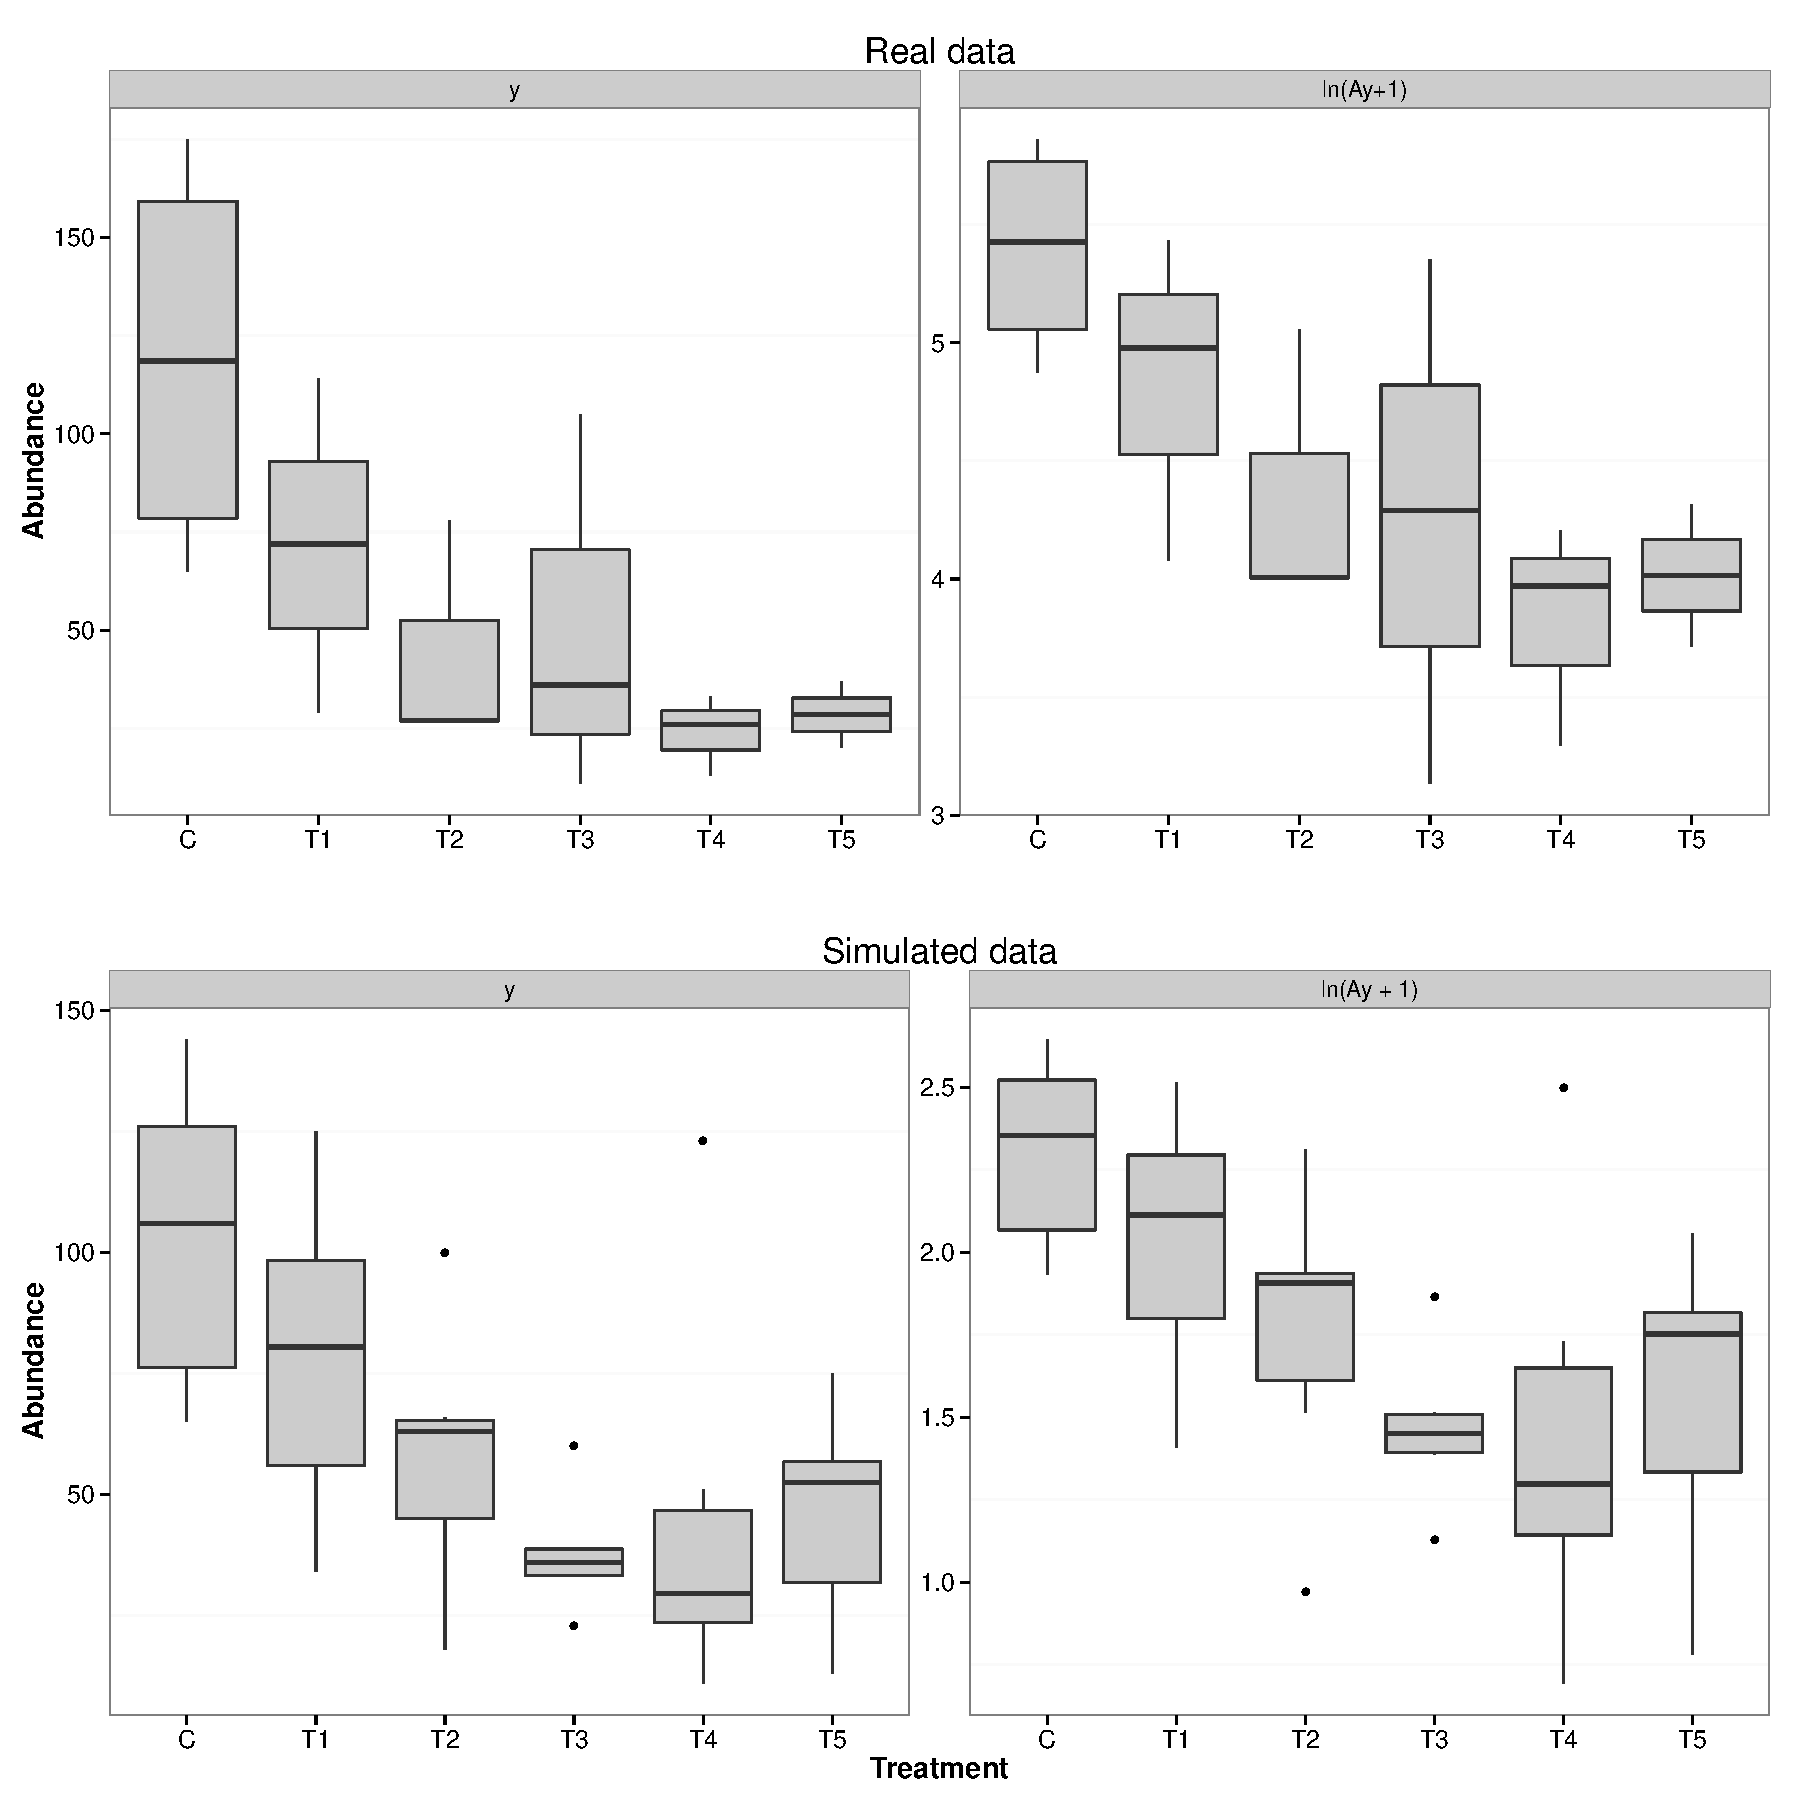
\includegraphics[width = \textwidth]{p4_1.pdf}
  \caption{Real data from Brock et al... (top) and one realisation of simulated data (below, N = 6, $\mu_c$ = 100). Left panel show raw counts, right panel $log(A \cdot x + 1)$ transformed counts.}
\end{figure}

\subsection{Simulations based on real data}

\section{Results}
\subsection{Simulation scenarious}

\begin{figure}
  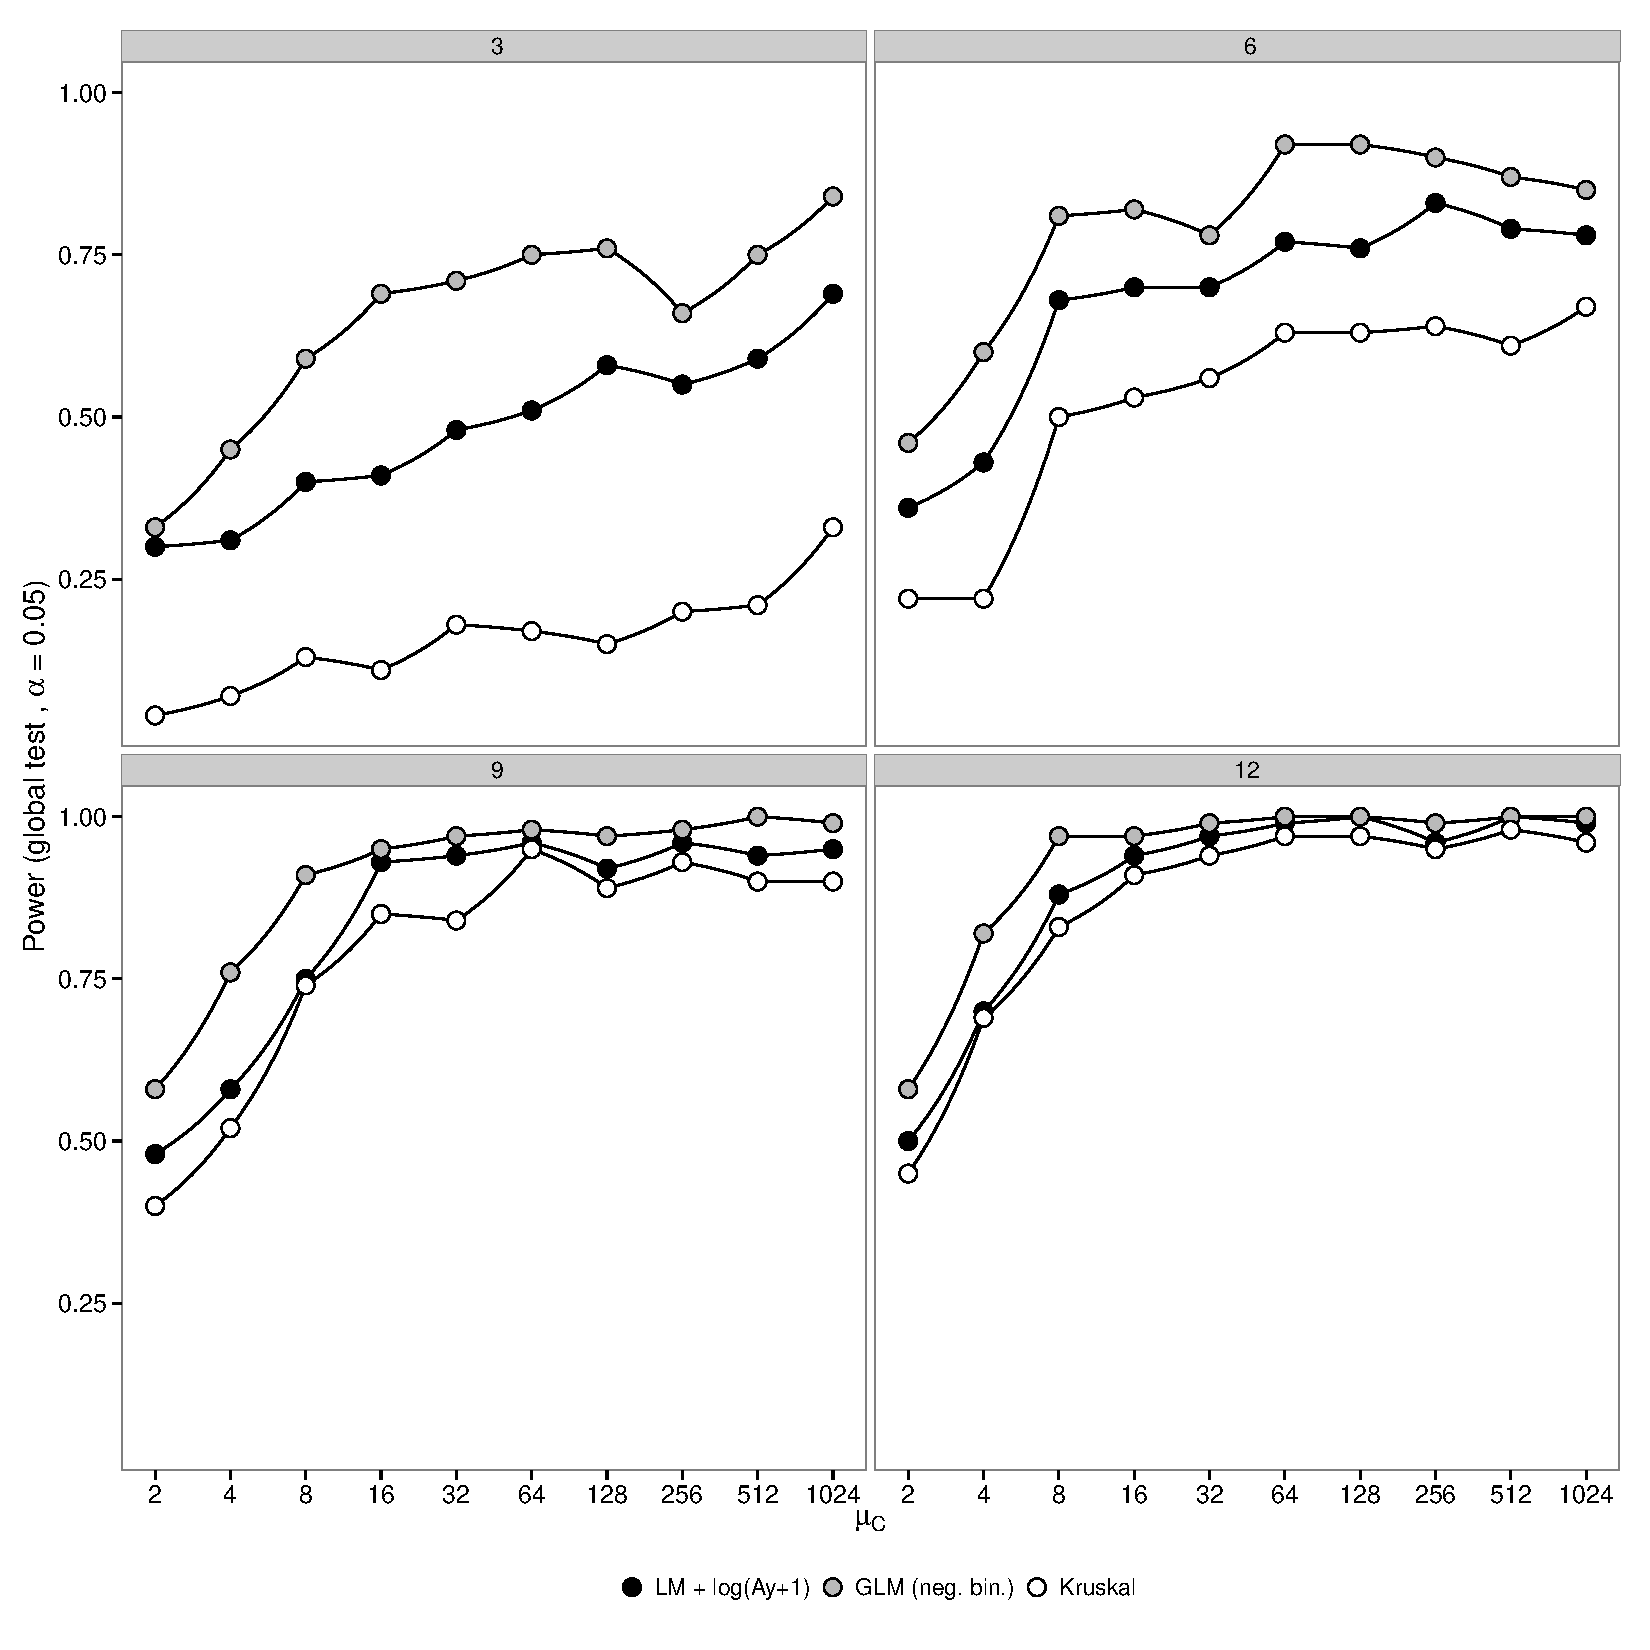
\includegraphics[width = \textwidth]{p2.pdf}
  \caption{Power.}
\end{figure}

\begin{figure}
  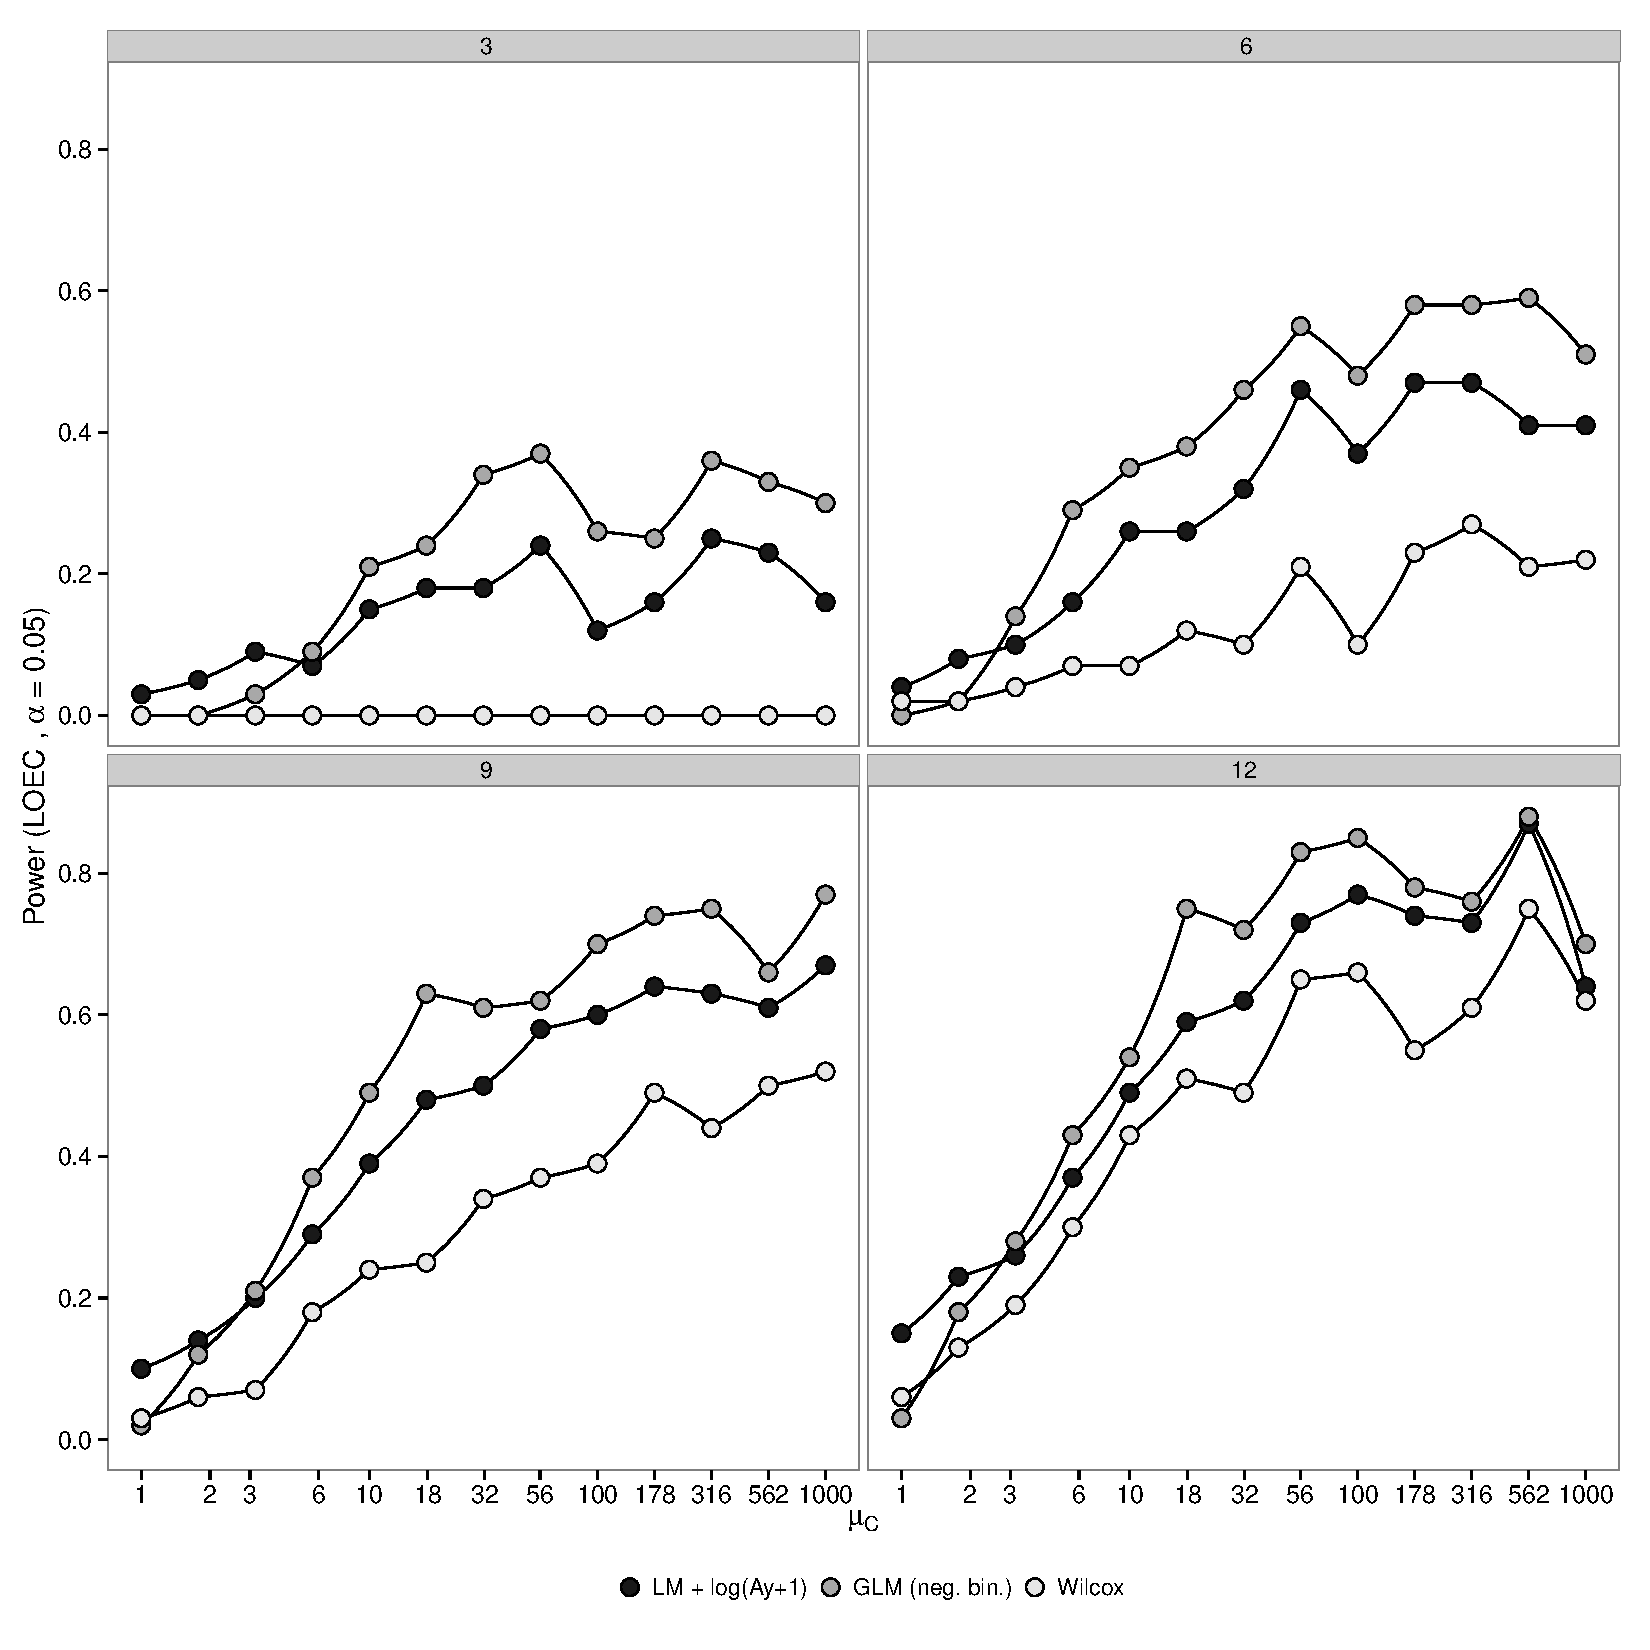
\includegraphics[width = \textwidth]{p3.pdf}
  \caption{Power to detect LOEC.}
\end{figure}

-> bei kleinerm muc lm besser weil annahmen nicht passen (checken)?

\subsection{Simulations based on real data}

\section{Discussion}

Decide between NB and P? - Mean-Var-Plot!

\section{Conclusion}

\appendix
\section{Tipps
(Or move up to introduction?)
Check distribution}


\section{TODO}
Read about nparcomp.




\end{document}
